\documentclass[UTF8]{article}
% 中文支持
\usepackage[UTF8]{ctex}	
% pdf调用 封面
\usepackage{pdfpages}
% color宏包
\usepackage{color}  
% 导入图片
\usepackage{caption}
\usepackage{graphicx, subfig}
% 防止图片乱跑
\usepackage{float}
% 支持数学符号
\usepackage{amsmath}
% 支持代码块
\usepackage{listings}
% pdf加入大纲
\usepackage{hyperref}
% 大纲去红框
\hypersetup{hidelinks,
	colorlinks=true,
	allcolors=black,
	pdfstartview=Fit,
	breaklinks=true
}

% 绘制三线表
\usepackage{booktabs}    
% 消除警告
\usepackage{lmodern}

% 绘图
\usepackage{tikz}
\usetikzlibrary{positioning, shapes.geometric}
\tikzstyle{bag} = [align=center]

% 设置页面的环境,a4纸张大小,左右上下边距信息
\usepackage[a4paper, left=31.8mm, right=31.8mm, top=25.4mm, bottom=25.4mm]{geometry}

% 代码块的基本设置
\lstset{
 breaklines,%自动换行
 columns=fixed,       
 numbers=left,                                        % 在左侧显示行号
 numberstyle=\tiny\color{gray},                       % 设定行号格式
 frame=none,                                          % 不显示背景边框
 backgroundcolor=\color[RGB]{245,245,244},            % 设定背景颜色
 keywordstyle=\color[RGB]{40,40,255},                 % 设定关键字颜色
 numberstyle=\footnotesize\color{darkgray},           
 commentstyle=\it\color[RGB]{0,96,96},                % 设置代码注释的格式
 stringstyle=\rmfamily\slshape\color[RGB]{128,0,0},   % 设置字符串格式
 showstringspaces=false,                              % 不显示字符串中的空格
 language=python,                                        % 设置语言
}

\usepackage{fancyhdr} % Headers and footers
\usepackage{lastpage}
\pagestyle{fancy} % All pages have headers and footers
% \fancyhead{} % Blank out the default header
\fancyhead[C]{网络过程控制系统课程报告:过程控制系统的智能化发展} % Custom header text

\begin{document}



hello world

% 两图片并排
% \begin{figure}[htbp]
% 	\centering
% 	\begin{minipage}{0.49\linewidth}
% 		\centering
% 		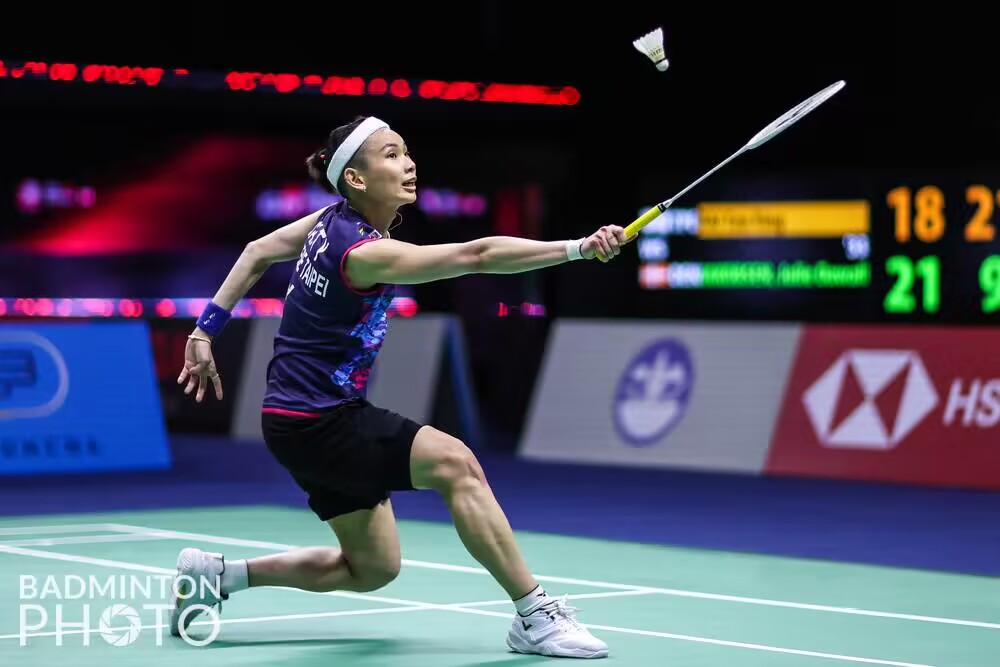
\includegraphics[width=0.9\linewidth]{figure/figure_1.jpg}
% 		\caption{title1}
% 		\label{label1} %文中引用该图片代号
% 	\end{minipage}
% 	%\qquad
% 	\begin{minipage}{0.49\linewidth}
% 		\centering
% 		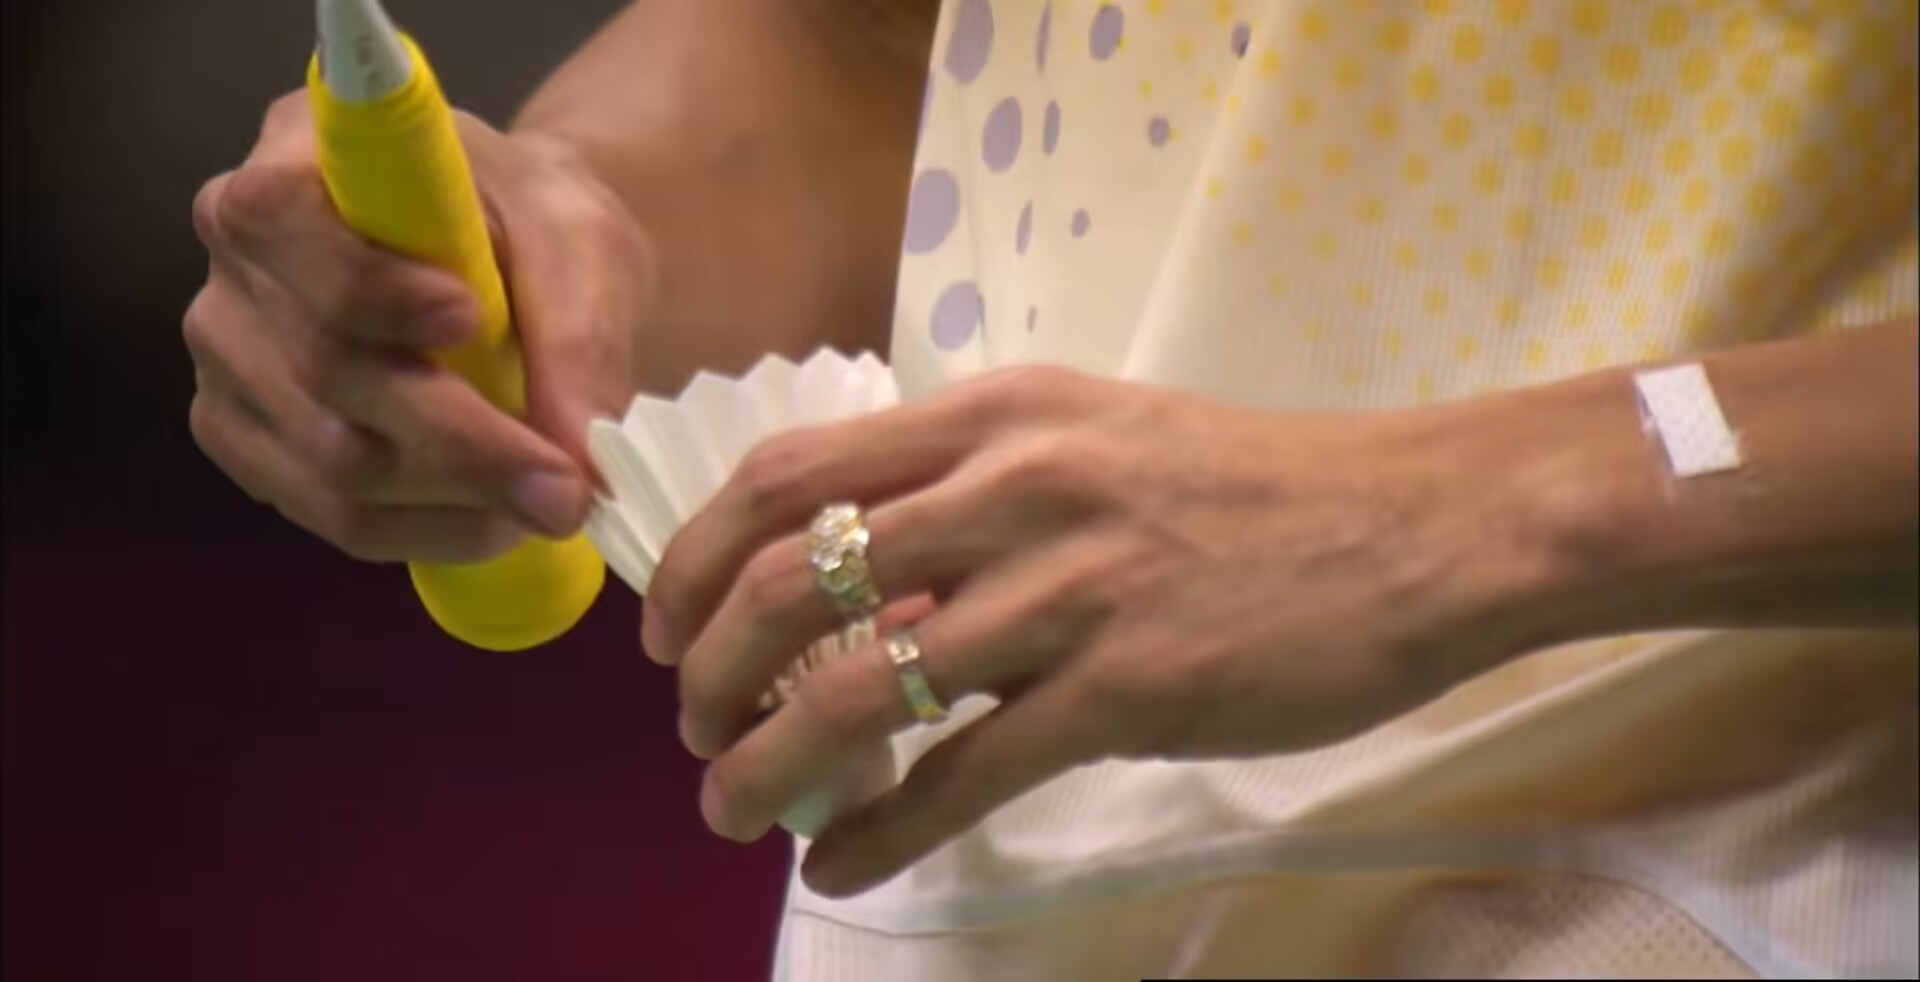
\includegraphics[width=0.9\linewidth]{figure/figure_3.jpg}
% 		\caption{title2}
% 		\label{label2} %文中引用该图片代号
% 	\end{minipage}
% \end{figure}

% \begin{titlepage}
% % 封面信息
% \includepdf[pages={1}]{cover.pdf}
% \end{titlepage}

% \begin{titlepage}
% % 封面信息
% \includepdf[pages={1}]{./cover/cover.pdf}
% \end{titlepage}

% 生成目录
% \tableofcontents
% \cleardoublepage

% 导入图片
% \begin{figure}[H]
%     \centering % 居中 
%     % 图片文件的相对路径
%     \includegraphics[width=.8\textwidth]{figure/exp1_1_model.png} 
%     \caption{Simulink模型} % caption是图片的标题
%     % \label{fig:img} % 此处的label相当于一个图片的专属标志,目的是方便上下文的引用
%     % 图片引用格式:\ref{fig:img} 可能需要二次编译
% \end{figure}

% 导入代码
% \begin{lstlisting}
% a
% \end{lstlisting}

% 重置章节编号
% \setcounter{section}{0}

% \begin{table}[H] % 防止表格乱跑
% \centering % 居中
% \begin{tabular}{cccccc} % 指明列数
% 	\toprule % 顶部粗线
% 	序号 & 姓名 & 性别 & 年龄 & 身高/cm & 体重/kg \\
% 	\midrule % 中间细线
% 	1 & 张三 & M & 16 & 163 & 50 \\ % 每行末尾都要加换行符
% 	2 & 王红 & F & 15 & 159 & 47 \\
% 	3 & 李二 & M & 17 & 165 & 52 \\
% 	\bottomrule % 底部粗线
% \end{tabular}
% \caption{title} % 标题
% \end{table}

% \begin{thebibliography}{99}  
% 	\bibitem{ref1} 《现场总线技术及应用教程(第二版)》,王永华,机械工业出版社
%   \bibitem{ref13} \href{https://www.elecfans.com/kongzhijishu/1080520.html}{工业控制系统未来的发展趋势分析}:https://www.elecfans.com/kongzhijishu/1080520.html
% \end{thebibliography}

\end{document}